\documentclass[11pt]{article}

%%%%%%%%%%%%%%Include Packages%%%%%%%%%%%%%%%%%%%%%%%%%%
\usepackage{xcolor}
\usepackage{mathtools}
\usepackage[a4paper, total={6in, 8in}, margin=1.25in]{geometry}
\usepackage{amsmath}
\usepackage{amssymb}
\usepackage{paralist}
\usepackage{rsfso}
\usepackage{amsthm}
\usepackage{wasysym}
\usepackage[inline]{enumitem}   
\usepackage{hyperref}
\usepackage{tocloft}
\usepackage{titlesec}
\usepackage{colortbl}
\usepackage{wrapfig}
\usepackage{pdfpages}
%%%%%%%%%%%%%%%%%%%%%%%%%%%%%%%%%%%%%%%%%%%%%%%%%%%%%%%%



\begin{document}
%\begin{wrapfigure}[8]{r}{0.3\textwidth}
%  \begin{center}
%  \vspace{-15pt}
%    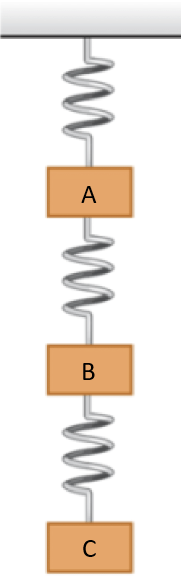
\includegraphics[scale=0.45]{springboxes}
%  \end{center}
%\end{wrapfigure}
\Large \noindent \textbf{Physics 1A Discussion (Week 7)}\\
\normalsize
Department of Physics and Astronomy, UCLA\\
\noindent\rule{8cm}{0.4pt}\\


\noindent \textbf{Problem 1}: Consider a moving box with initial momentum $\vec{p} = (-3.00, 4.00)$\, kg\,m/s. A time-dependent force $\vec{F}(t) = (0.280t, -0.450t^2)$\,N is applied to the box starting at time $t = 0$ seconds. Find the magnitude of momentum of the box at time $t = 2$ seconds.\\

\newpage
\noindent \textbf{Problem 2}: 
There was a traffic accident happened at the intersection below. The yellow car (car A) with a mass of $m_A=2000$\,kg was going from west to east at a speed $v_A=35$ miles per hour. The red car (car B) with a mass of $m_B = 1500$ kg was going from south to north with some unknown speed $v_B$. As a result of the collision, the cars were stuck together and subsequently moved as one object towards the direction as shown in the figure, at an angle $60^\circ$ north of east. Neglect friction in this problem. 

\begin{center}
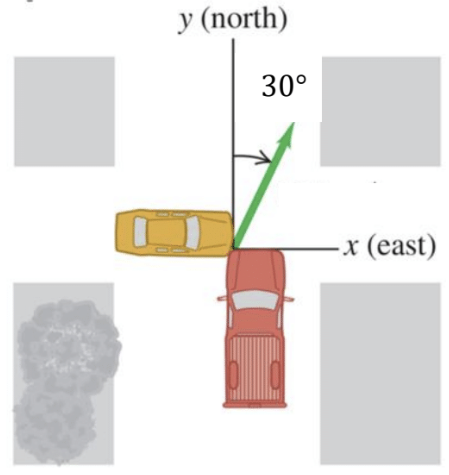
\includegraphics[scale=0.39]{cars}
\end{center}

\noindent The speed limit was 50 miles per hour. Determine whether car B was speeding.

\newpage
\textbf{Problem 1}: This is a straightforward calculus computation. From the definition of momentum,
\begin{align*}
\Delta \vec{p} = m \, \Delta \vec{v} = m \int \vec{a}\, dt = m \int \frac{\vec{F}}{m}\, dt = \int \vec{F}\, dt\,,
\end{align*}
where we have employed Newton's second law $\vec{F} = m\vec{a}$. Now with the time labels, 
\begin{align*}
\vec{p}(t=2) = \vec{p}(t=0) + \int_0^2 \vec{F}\, dt\,.
\end{align*}
We calculate the $x$- and $y$-components separately, 
\begin{align*}
p_x(t=2) = p_x(t=0) + \int_0^2 F_x\, dt = -3 + \int_0^2 0.28t\, dt = -2.44\,.
\end{align*}
\begin{align*}
p_y(t=2) = p_y(t=0) + \int_0^2 F_y\, dt = 4 + \int_0^2 -0.45t^2\, dt =2.8\,. \end{align*}
Therefore, at time $t = 2$ seconds, we have $\vec{p} = (-2.44\,, 2.80)$\,kg\,m/s. The magnitude of this momentum vector is
\begin{align*}
p = \sqrt{(-2.44)^2 + (2.8)^2} = 3.71\,\text{kg\,m/s}\,.
\end{align*}

\textbf{Problem 2}: Most of the collision problems should be solved by using conservation of momentum, which is the statement that momentum is conserved along each of the axes in a coordinate system. In this case, we set up the $x$-axis in the west-to-east direction, and the $y$-axis in the south-to-north direction. Along the $x$-direction, 
\begin{align*}
p_{A,x} + p_{B,x} = p_{AB,x}\,,
\end{align*}
where $\vec{p}_A$ and $\vec{p}_B$ are the momenta of the cars before collision, and $\vec{p}_{AB}$ is the momentum of the two cars stuck together after the collision. Similarly in the $y$-direction, 
\begin{align*}
p_{A,y} + p_{B,y} = p_{AB,y}\,.
\end{align*}
Now we only need to use the definition $p = mv$ to write out the equations, and solve the the unknowns. 
\begin{align*}
p_{A,x} + p_{B,x} &= p_{AB,x}\,,\\
m_A v_{A,x} + m_B v_{B,x} &= m_{AB} v_{AB,x}\,,\\
(2000)\, (35) + (1500)\, (0)&=  (2000+1500)\, v_{AB} \cos(60^\circ)\,.
\end{align*}
\begin{align*}
p_{A,y} + p_{B,y} &= p_{AB,y}\,,\\
m_A v_{A,y} + m_B v_{B,y} &= m_{AB} v_{AB,y}\,,\\
(2000)\, (0) + (1500)\, v_B&=  (2000+1500)\, v_{AB} \sin(60^\circ)\,.
\end{align*}
Notice that I did not convert mph to meters per second for the velocities, this is because the conversion is equivalent to multiplying each equation by the same conversion factor. Now I have a system of two equations with two unknowns $v_B$ and $v_{AB}$,
\begin{align*}
\begin{cases}
2000\cdot 35 = 3500 v_{AB} \cos(60^\circ)\\
1500 v_B = 3500 v_{AB} \sin(60^\circ)
\end{cases}\,.
\end{align*}
Solving this system we obtain 
\begin{align*}
v_B = \frac{2000\cdot 35}{1500}\tan(60^\circ)=80.8\,\text{mph}\,.
\end{align*}
In fact, car B was a speeder. 

\end{document}


